\section{Narvis: System Design and Implementation}

% Thus, it has two kinds of users: editors, the data visualization experts who use Narvis to create an explanation slideshow, and audiences, the general audience who watch the slideshow created by ediors.

Guided by the theory model discussed in section3, as well as the design consideration mentioned in section 4, we desing and implement Narvis, an authoring tool for crafting slideshows for the presentation of visualization. The workflow of Narvis consists of three phases (Figure \siwei{ref}), i.e., Automatic Analysis Phase, Manual Editing Phase, and Viewing Phase.

% The workflow of Narvis includes three phases (Figure \siwei{ref}):  In Automatic Analysis Phase, the system accepts the input visualization, extracts graphical elements and classifies them into groups for further edit. 
% In Human Editing Phase, editors will be involved to modify the output from the Automatic Analysis Phase, and use the templates Narvis provide to craft a explanation slideshow. 
% In Reviewing Phase, audience can assess the slide show generated in Human Editing Phase. Their click activity and comments will be recorded and send to the editors, helping them improve the quality of the slide show. 

\begin{figure}
 \centering % avoid the use of \begin{center}...\end{center} and use \centering instead (more compact)
 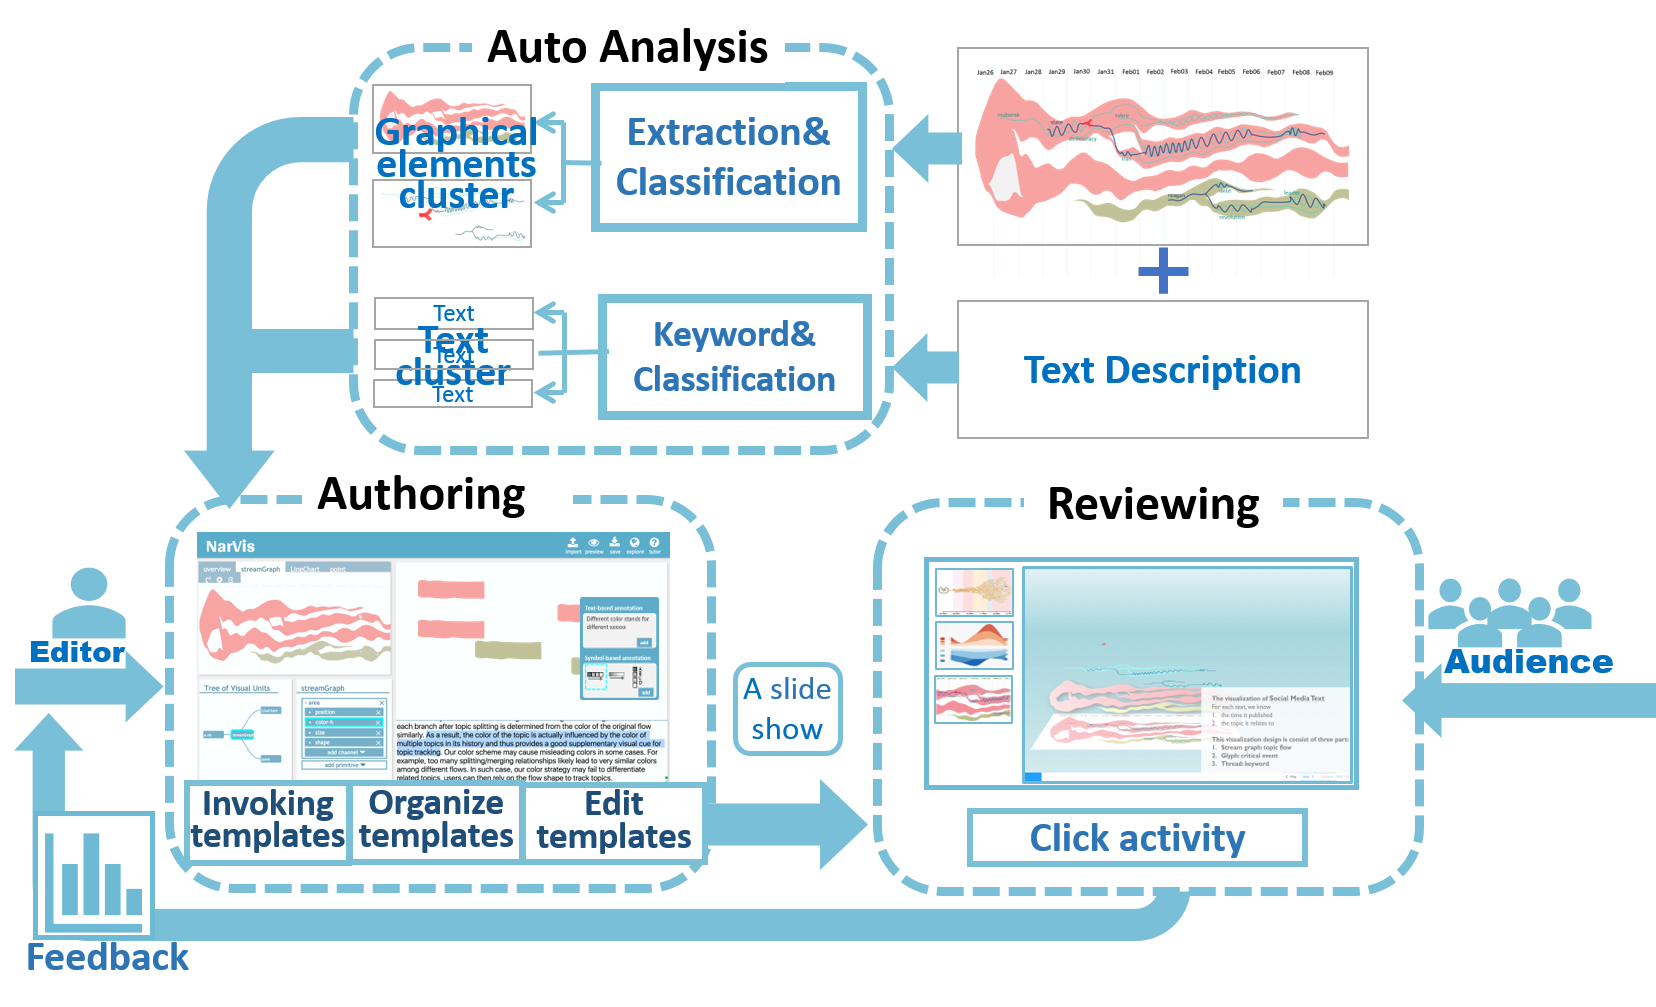
\includegraphics[width=\columnwidth]{overview}
 \caption{The system overview}
 \label{fig:overview}
\end{figure}

\subsection{Phase1: Auto Analysis}

% The auto analysis has two parts: one for input image and one for input text. It automatically extract the graphic elements and divide them into different cluster, facilitating later editing.(DE1) Note that the textual input is not necessary but it provides hints when editors add annotations manually in the Human Editing Phase.(DE1)

The input of Narvis includes two parts: one image presenting a visual design (mandatory) and a piece of text describing the design (optional). In this phase, Narvis accepts the input image and extracts graphical elements to facilitate further authoring. If a textual description is provided, Narvis groups these sentence based on a keyword detection method, and each sentence group is tagged as descriptive of a certain visual grammar.

\subsubsection{Analysis of input image}
% The auto analysis of input image has three main steps. It first detects all primitives that it finds in the given image and also detects any labels that are present in the visualization. It will then cluster objects that are spacially linked and extract non-target objects. Finally, it will fill in any empty spaces left inside objects from extraction with the appropriate color so as to show the target object in its entirety.
The analysis of input image includes three steps, i.e., object detection, object clustering and object recovery.

% The first step, object detection, is done by iterating through all the pixels on the bitmap. 
\textbf{Object detection.} Narvis iterates through all pixels in the input image. At every iteration, we first check to see if this pixel has already been tagged as part of an object. If not, we know that this pixel forms \siwei{a part of a new object.} We explore the colors of the neighboring pixels, where the neighbors are chosen such that the distance between the current pixel and a potential neighbor \siwei{is less than 3}. If the difference in color between a neighbor pixel and the current pixel is less than a threshold, the neighboring pixel is tagged as part of the same object. Once all neighbors have been classified as either part of the same object or not, we choose another pixel that was classified as part of the same object and apply this algorithm again. This is a modified BFS algorithm and allows us to identify all unique ojects in the given visualization.

\textbf{Object clustering.} Once all the objects have been detected, we have to extract a target object. To extract an object means to only select the pixels that are classified as part of this object, so we should remove all objects that are not part of this object and we should extract objects that are inside our target object.It is trivial to set all pixels that are not within or part of our object to have color white. For objects that are inside our target object, i.e. those objects that are clustered with out target object, we will first detect that object then programmatically change its pixels to white.

\textbf{Object recovery.} Once we have completed extraction, we have the issue of these white spaces. The reason this is an issue is because an extracted object might have been dividing two objects, and so when it is extracted, we lose the boundary between our target object and another object, which can cause confusion as to whether that white space should be colored in or not. To solve this boundary problem, we create a queue of the white spaces, with each data point giving the starting and ending point of that space. We then look at the intervals between enclosed white spaced objects, if that interval is above a threshhold, we take that white space to not be part of our object. If it is below our threshhold, then we enclose the white space with the target objects color, creating a boundary for it. The main difference is that for objects not within our target object, we do not create a boundary, whereas objects within our target object are enclosed with the target objects color.

\subsubsection{Analysis of input textual description}
For the input textual description, we offer a basic text detection and classification algorithm, which uses a dictionary of terms that are highly correlated with certain channels. E.g. the word "length" is highly correlated with the size channel. To do the text detection, we first classify each sentence depending on whether it contains any of the key words in our dictionary. If it contains a key word for one of the channels, the sentence is tagged as being a description of that channels visualization. Once we have tagged all the sentences, whenever a channel is selected, we show the entire text that was inputted and highlight the text that has been tagged as descriptive of that channels visualization.

The algorithm we proposed is a compromise between efficiency and performance. At this time point, it is limited to images with high quality and clear edges, but its performance can be improved by adopting other well-established algorithm, such as the algorithm based on patch detection and clustering \cite{savva_revision:_2011} and the algorithm based on edge maps \cite{huang2003model}.

\subsection{Phase2: Manual Editing}
In Narvis, editors craft an introduction slideshow by constructing build-in blocks called as templates in Narvis.(DE1) We first introduce the workflow of this phase, which includes three steps, i.e., invoking templates, organizing templates and modifying templates, as illustrated in Figure \siwei{ref}. Then ,we explain how we design and organize the templates in Narvis. \siwei{sth}
% We introduce three panels in this phase acting as three steps in the workflow to allow editors  

\subsubsection{Invoking Templates} 

After graphical elements are extracted and clustered based on visual representation, each cluster appears as a tabbed panel in the \textit{Source Panel} (Figure \siwei{ref}). 

Editors can switch between these tabbed panels, add, delete, split, or merge graphical elements in each panel, making sure that 1) all the graphical elements of the same visual unit is in the same panel 2) every graphical element belongs to one and only panel. Then, for each visual unit, the user invokes an associated template from the library. For example, for the tabbed panel in \siwei{fig}, the editor should call a ``scatter plot'' template.

The relationship between graphical elements and templates is similar to the one between data and function. Templates contain a set of operations to produce a sequence of slides from the input graphical elements.  (DE1, DE2) 

\subsubsection{Organizing Templates} 
Once invoked, a template will show on the \textit{Tree Panel} as a tree node. 
Editors are allowed to adjust the relationships between invoked templates through interacting in the \textit{Unit Tree} panel, where all visual units are shown as tree nodes.
By dragging and dropping these nodes, editors organize the structure of the tree diagram, which reflects the relationship between visual units and determines the narrative sequence of the slideshow. The same tree diagram will shown on the produced slideshow, severing as a progress bar to give the audience a sense of overview. (DA.6)

\subsubsection{Modifying Templates} 
% \textbf{\textit{ Unit Panel \& Editor panel}: personalized modification}
% but it also allow the users high flexibity to modify these temples, thus guaranteeing the expressiveness of this system. 
Narvis provides templates to generate slideshows with high efficiency. 
It also supports flexible modification of templates for expressiveness.
Editors can edit a template in the \textit{Unit Panel} by selecting a node on the \textit{Tree Panel}. In each template, all possible visual grammar are enumerated. Editors can delete unused one themselves, thus eliminating the unconscious omission of crucial information (DA.5). It also recommends a narrative sequence of visual grammars, based on the metrics we mentioned in section 3.1.4 (DE1, DA3, DA5). 
In the \textit{Editor Panel}, with the hints from Narvis, editors add annotations to facilitate graph and chart comprehension. For each slide, Narvis offers questions or sentence with blank for adding text-based annotation, and a list of suggested design options for symbol-based annotation. \siwei{Fig}

\subsubsection{A Library of Templates}
We propose a library of templates for the narrative explanation of a visualization. A template is a set of slides that tends to introduce an visual unit, which can be descibed as an orthogonal combination of visual primitives and construction rules, as shown in tab.1. Since advanced visualization design is the assembly of miscellaneous visual units, we conjecture such templates can achieve a high level of efficiency for the explanation of a visualization. (DA1)Meanwhile, allowing users a high flexible, friendly interface to edit offered templates, Narvis maintains a considerable level of expressiveness and accessibility. 

\textbf{Types of templates}

Narvis use a 8*3 table to organize the provided templates, as shown in \textbf{fig}. Narvis is extensible, new templates can be added by its developer through programming, or by end users through uploading their modified templates. At the same time, all newly added templates are classified into a certain cell of the 8*3 matrix, so as to avoid overwhelming users with a cornucopia of confusing options.

\textbf{Templates design}

We apply the analysis and theory model in section 3 for the design of templates. A template has four core components: 1) a well-considered narrative sequence for visual grammar explanation; 2) exaggeration or suppression of certain visual channels in some slides; 3) a series of narrative techniques such as attention cues, animated transitions, information repetition, to orientate visual attention and facilitate perception;(DE.1) 4) Hints for adding annotations (DE.2) in each slide(DA.4)

With a visual unit, more specifically, a set of graphic elements, as input, a templates will generate a slideshow and each slide is responsible for the explaining of one visual grammar.(DA.4) These slides are sorted based on the narrative sequence we discussed in section 3.3. In each slide, we offer hints to guide the annotation process. These hints are sentence with blanks to fill in, heuristic questions, or a list of suggestion symbols. A visual channel is suppressed until its grammar has been explained. For example, before we introduce the visual grammar of color, all the object will be gray.  The graphical elements in different slides, which might have different visual appearance due to the applied exaggeration or suppression of visual channels, are perceptively connected through morphing animation.

\textbf{Animation embedded in templates }

Narvis provides 8 types of animation, implement them in templates based on their effects on human attention and perception(DA.1), which has been widely discussed in previous work.\cite{robertson_effectiveness_2008, waldner_attractive_2014, heer_animated_2007}We also provide a novel decomposition animation at the beginning of the introduction slideshow to engage the audience as well as to help them get a sense of overview.(DA.6)

\begin{table}[tb]
  \caption{A summary of animation provided}
  \label{tab:animation}
  \small
  \centering
  \begin{tabular}{p{1cm}|p{0.9cm}|p{0.9cm}|p{0.9cm}|p{1.5cm}|p{0.9cm}}
  \toprule
 \textbf{Animation} &\textbf{Engaging} & \textbf{orientate attention} & \textbf{perception} &\textbf{working scenario} &\textbf{ref} \\ 
  \midrule
  \textbf{Morphing} &\checkmark & \checkmark &\checkmark & grammar of size, grammar of shape & \cite{ruchikachorn_learning_2015, heer_animated_2007} \\ 
  \midrule
  \textbf{Blur} &   &\checkmark  &   & focus+context & \cite{pinto2008selecting}\\ 
 \midrule
  \textbf{Flicker} & & \checkmark &  & focus &\cite{waldner_attractive_2014} \\
  \midrule
  \textbf{Motion} & \checkmark & \checkmark & \checkmark & grammar of position & \cite{huber_visualizing_2005} \\
  \midrule
  \textbf{Zoom-in/out} & \checkmark &\checkmark &  & focus&  \\
  \midrule
  \textbf{Annotation} &  & \checkmark &\checkmark &   textual explain & \cite{segel_narrative_2010 } \\
  \midrule
  \textbf{Fade in/out} &  & \checkmark &  & & \\
  \midrule
  \textbf{Decompose} & \checkmark &  &\checkmark & Show how a visualization is composed by visual units & A novel design by us \\
  \bottomrule

  \end{tabular}
  \vspace{1mm}
\end{table}


Animation is a double-edge sword, which introduces both benefits and pitfalls. We are not discussing the effects of animation here. Editors can choose to remove these animation if they prefer an abstract slide show or they are suspicious of the effects of animation. 


\subsection{Phase3: Viewing}
\subsubsection{The interface for audience}
The interface of audience is composed of two panels.

\textbf{\textit{Gallery Panel:}the collection of generated slide show}
 
\textit{Gallery Panel} exhibit all the slideshows produced by editors and saved in Narvis. Every slideshow is presented by an image, the visualization it tends to explain. By clicking on the image, users can watch this slideshow in the \textit{Screen Panel}. 

\textbf{\textit{Screen Panel:}  review and comment}
Every slide show displayed in \textit{Gallery}is a series of slides, each of which is responsible for the delivery of one simple encoding information, for example, the horizontal position indicates time. In the \textit{Screen} panel, users click buttons to move forward or backward to view these slides, and their click activity will be recorded automatically by Narvis. 
\subsubsection{Generated Report}
The report visualizes the click activity of audience in the form of a stacked bar chart, as\textbf{fig}. The heigh of the bar indicates the time spent on watching this slide. If audiences go back to a previous slide while viewing, a bar will be stacked on the top of the previous one. If there are animation in the slide show, a white line will be drawn upon the bar chart, referring to the animation playing time of each slide, thus gives a judgement whether an animation is too fast or too slow. (DE.3)
\subsection{Iterative Design}
To investigate the usability of Narvis, we invited 4 UGs from diverse backgrounds to watch an introduction slideshow produced by a data visualization professor with Narvis. 
Based on their feedback, we iterate over the design of Narvis as follow:
\subsubsection{An compulsory Introduction}
In the initially design, an introduction slideshow is purely the combination of templates. In other words, it straightforwardly explain each visual units after an overview of the visualization. However, the participants complained that they are less motivated to learn a visual design without an awareness of the background. Questions like, \textit{what's the motivation of this visual design}, \textit{what's the dataset}, and \textit{what kinds of problems it can solve} need to be answered before the introduction of this visual design. Thus, we add a compulsory introduction slide at the beginning of each slideshow, which is displayed as a root node of the tree diagram in \textit{Tree Panel}. This slide contains questions that guide the editors to give a brief description of the background.
\subsubsection{Different Levels of Detail}
While 3 UGs appreciate this detailed introduction slideshow, and consider the animation applied as engaging and enjoyable. Another UG, who has taken a data visualization course before and is familiar with some visualization designs, thought some slides and animation are redundant. 
Thus, we offer 3 levels of details which the audience can choose from. The detailed one displays all the animation, the normal ones skip the animation for some simple visual grammar such as color and size, and the abstract one discards all animation and put the annotation for color and size in one slide
    
\subsection{A Working Scenario}
Jessica has extensive experience in the field of data visualization, and has implement a visual analytics tool in a review service website based on the design of OpinionSeer\cite{wu_opinionseer:_2010}. To help audience better understand this design, she needs to publish a tutorial accompanied with it.
First, she loads the screen-shot of her system, as well a textual description, into Narvis.
After a few seconds, the system automatically extracts the graphics elements and clusters them based on features. As Figure\siwei{ref} shows, Jessica obtains four clusters. 

Then, she defines visual units based on clusters. By default, each cluster includes all graphics elements belonging to one visual unit. However, she observes that geographic ring and calendar ring are in the same cluster due to their similar appearance. Therefore, she divides it into two clusters, containing geographic ring and calendar ring respectively.
% then refines the clustering results, making sure every graphic elements in one visual unit is put in one cluster \textbf{figure xxx}. Finally she obtains four clusters.

Next, she chooses narrative templates for each visual unit. 
%Some visual units, such as the triangle scatter plot, are novel and no narrative template in the library is able to match. Therefore, Jessica chooses the template of regular scatter plot for best match.
% for triangle scatter plot, which differs from the triangle plot in the encoding of position. 
Moreover, Jessica edits the narrative templates based on her design. 
% In the templates, we enumerate all the possible visual encodings. 
She goes through all four templates in the ``\siwei{what is in-unit}in-unit'', and deletes the visual channels with no encodings, such as \siwei{sth}. 
Through drag and drop, Jessica further organizes the structure of the unit tree based on the relationships between units. For example, \siwei{some example}

Jessica further improves the quality of animation by adding annotations and strengthening the binding between data and graphic elements. 
% When adding annotation to a certain channel, the related text will highlight in the text area, aiming to offer a better user experience.   


To refine the readability of the tutorial, Jessica asks several friends, who have no experience in data visualization, to watch the tutorial before release. Narvis collects their viewing behavior from click activities, generates statistics results, and visualize it in the form of stacked bar chart , which helps Jessica answer questions like \textit{``which slides do they skip?''}, \textit{``which slides do they review several times?''}, and \textit{``which slides do they stay for a long time?''}.
% These click sequence data provides cues for Jessica to strengthen and refine the readability of the tutorial. 

% revealing information such as, ,   



